The \peripheral{SYSTEM} peripheral manages a potpourri of system-level blocks, including the MCU clocks, interrupt control, watchdog timer, and a CRC data verification module.

\subsection{System Clocks and Clock Management} \label{ss:clocks}
The MCU has four clock sources: HFXT, LFXT, DCO0, and DCO1. HFXT and LFXT are external clock sources, which must be provided to the MCU via the \pin{ClkHFXT} and \pin{ClkLFXT} pins, respectively. DCO0 and DCO1 are internal, programmable frequency clock sources provided by digitally controllable oscillator circuits.

The Myshkin MCU is designed and characterised for operation with a maximum clock frequency of 24~\si{\mega\hertz}. HFXT should therefore not exceed 24~\si{\mega\hertz}. LFXT is suggested to be exactly 32.768~\si{\kilo\hertz} to provide an accurate method of measuring time. The frequencies of DCO0 and DCO1 are configured with the \register{DCO0BIAS} and \register{DCO1BIAS} registers; higher bias values produce higher frequencies.

\textbf{Note on overclocking:} It is possible to operate the Myshkin MCU beyond 24~\si{\mega\hertz} by supplying a higher-frequency signal on the \pin{ClkHFXT} pin or by configuring the internal DCOs to produce frequencies above 24~\si{\mega\hertz}. As with any digital circuit operated beyond its rated frequency, doing so may produce setup-time violations, incorrect computational results, and unpredictable behaviour. Operation above 24~\si{\mega\hertz} is \textbf{not guaranteed} and is undertaken entirely at the user's risk.

Two clocks, the main clock (MCLK) and the submain clock (SMCLK), form the roots of the MCU clock tree, shown in Figure \ref{fig:mcu-clock-system}. MCLK and SMCLK can each select one of the four source clocks as their base and optionally divide the frequency further using \register{CLKDIVCR}. MCLK drives the CPU, while SMCLK drives most of the peripherals. Both clocks use glitch-free multiplexers to prevent spurious transitions when switching sources.

MCLK cannot be turned off, but SMCLK and individual source clocks can be independently disabled via \register{SYSCLKCR}. DCO0 and DCO1 are off by default and must be explicitly powered on by setting \bitfield{DCO0ON} or \bitfield{DCO1ON}. HFXT and LFXT are enabled by default and may be disabled with \bitfield{HFXTOFF} and \bitfield{LFXTOFF}. If a source clock is currently selected by MCLK or SMCLK, that source will be automatically kept enabled regardless of its disable bit in \register{SYSCLKCR}.

\begin{figure}[htpb]
\centering
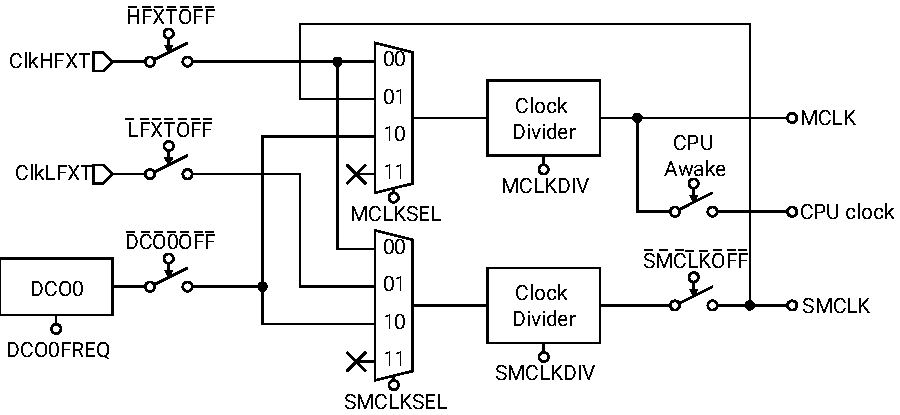
\includegraphics{figures/clocks-myshkin-2025-11.pdf}
\caption{MCU Clock System}
\label{fig:mcu-clock-system}
\end{figure}



\subsection{Power Saving Features} \label{ss:power-saving}
The MCU has several power-saving features.

The CPU is the most power-hungry part of the MCU, and its dynamic power consumption is proportional to the CPU clock frequency. Reducing the frequency of MCLK is the primary avenue for reducing total dynamic power consumption. This can be done by utilising the MCLK clock divider in \register{CLKDIVCR}, by switching MCLK to a lower-frequency source via \bitfield{MCLKSEL}, or by reducing the frequency of the currently-selected source. The internal DCOs offer a wide range of programmable frequencies through their bias settings and can be used as a low-power clock source when HFXT is disabled.

Another method to save power is to turn off unused clocks. Remember, however, that the \pin{ClkHFXT} pin is required to be a valid clock signal while the MCU boots. Failure to provide a valid clock may cause the chip to boot improperly, or not at all. For this reason, the start-HIGH pin(s) (\pin{SHx}) have been provided. On the PCB, the start-HIGH pins should be connected to the enable input of the external clock source driving \pin{ClkHFXT}, ensuring the clock is always present during reset. After boot, the user may switch MCLK to another source and then safely disable \pin{ClkHFXT}.

The static (leakage) power can be reduced by powering off unused on-chip memory blocks with \register{BLOCKPWR}. The ROM and RAM blocks include power-gating circuitry that physically disconnects their supply rail. The ROM can be powered down by setting \bitfield{ROMOFF}, and the two RAM blocks by setting \bitfield{RAM0OFF} and \bitfield{RAM1OFF}, respectively. Each powered-down block reduces leakage. Any access to a powered-down block will fail and produce undefined results. The entire contents of a RAM block are lost when it is powered down; data are undefined when it is powered back on until explicitly overwritten. Care must be taken to track the power state of each block to avoid undefined behaviour.



\subsection{CPU Sleep Mode} \label{ss:sleep}

Another way to conserve power is to run the CPU only when needed and switch it off when idle. Because the CPU accounts for the majority of dynamic power, duty-cycling its clock can yield significant savings. Peripherals can continue to operate while the CPU sleeps and may wake it when events occur. Long-term average CPU power is:
$$P_\textrm{CPU} = P_\textrm{CPU,\,100\%} \times \frac{t_\textrm{on}}{t_\textrm{on} + t_\textrm{off}}$$

Sleep mode is activated with the custom \asminline{sleep} instruction, which gates off the CPU clock and reduces its dynamic power to zero. The CPU can only be woken by an interrupt or a system reset. When an interrupt fires, the CPU clock is re-enabled for the duration of that interrupt service routine (ISR). Once all pending interrupts have been serviced the CPU returns to sleep, unless one of the ISRs executed the custom \asminline{wake} instruction, in which case the CPU remains awake and returns to the point in the main program where it went to sleep.

A code example to put the CPU to sleep is included in Listing \ref{lst:sleep}.

\begin{lstlisting}[style=customC, label=lst:sleep, caption={Example program to use CPU sleep mode}]
/** Includes **/
#include <MemoryMap.h>
#include <irq.h>

/** Interrupt Service Routine Declaration Macros **/
RVISR(IRQ_TIMER1_VECTOR, ISR_TIMER1)

/** Main Function **/
int main()
{
	// Set up TIMER1 here

	// Enable interrupts by unmasking them
	enable_all_interrupts();

	// Go to sleep
	cpu_sleep();

	// Insert code to execute after ISR wakes the CPU

	// Wait forever
	while (1) {}
}

/** Interrupt Service Routines **/
void ISR_TIMER1()
{
	// Do ISR processing here

	// Wake the CPU
	cpu_wake();
}
\end{lstlisting}



\subsection{CRC Module}
The CRC module enables the computation of a CRC16 checksum over an array of bytes. The checksum can be used to verify the integrity of data in a communication channel or in memory.

The module implements the CRC16-CDMA2000 standard with the following parameters:
\begin{itemize}
\item CRC width: 16 bits
\item Polynomial: \texttt{0xC857}
\item Initial value: \texttt{0xFFFF}
\item No output XOR
\item No input reflection
\item No output reflection
\end{itemize}

To compute a CRC over a byte array, first write \texttt{0xFFFF} to \register{CRCSTATE} to initialise the accumulator. Then write each byte of the array sequentially to \register{CRCDATA}; each write updates the running CRC. After the last byte has been written, read \register{CRCSTATE} to obtain the final CRC16 value.



\subsection{Interrupt Control}

The \peripheral{SYSTEM} peripheral manages global interrupt control. The \register{IRQCR} register contains the global interrupt enable bit \bitfield{IRQGEN}, which must be set before any interrupt can fire. It also contains \bitfield{IRQRECEN}, the interrupt recursion enable, which permits a running ISR to be preempted by a higher-priority interrupt when set.

Individual interrupt enables are controlled through the three 32-bit registers \register{IRQENL}, \register{IRQENM}, and \register{IRQENU}, providing enable bits for up to 96 interrupt vectors (83 are used on the Myshkin MCU). Each bit position corresponds directly to an IRQ vector number. An interrupt request will only trigger its ISR if both its individual enable bit and the global enable \bitfield{IRQGEN} are set.

Interrupt priority is managed through the three 32-bit registers \register{IRQPRIL}, \register{IRQPRIM}, and \register{IRQPRIU}. Each bit determines the priority tier of the corresponding IRQ: a \textbf{0} places the IRQ in the high-priority tier, a \textbf{1} places it in the low-priority tier. Within each tier, lower IRQ vector numbers carry higher priority. A high-priority interrupt (bit = 0) will always preempt a low-priority ISR (bit = 1) that is currently executing, regardless of vector number. Interrupt nesting to arbitrary depth is supported when \bitfield{IRQRECEN} is set, limited only by available stack space.



\subsection{Watchdog Timer}

The watchdog timer improves system reliability by automatically taking corrective action if software fails to service the watchdog within a configurable timeout period. The watchdog is controlled by \register{WDTCR}, which is write-protected and must be unlocked via \register{WDTPASS} before any configuration change.

The watchdog uses a 24-bit up-counter that increments on every MCLK cycle when enabled via \bitfield{WDTEN}. The timeout period is selected by \bitfield{WDTCDIV}, which chooses which bit of the counter triggers the watchdog event. A watchdog event occurs on the 0-to-1 transition of the selected bit, giving a timeout of $2^{\texttt{WDTCDIV}+16}$ MCLK cycles. At 24~\si{\mega\hertz} the timeout ranges from approximately 2.73~\si{\milli\second} (\texttt{WDTCDIV = 0000}, bit 16) to approximately 89.5~\si{\second} (\texttt{WDTCDIV = 1111}, bit 31).

On a watchdog event, the response depends on the configuration:
\begin{itemize}
  \item If \bitfield{WDTIE} is set \textbf{and} the watchdog IRQ is enabled in \register{IRQENL}, the watchdog ISR executes. If \bitfield{WDTHWRST} is also set, the system resets immediately after the ISR returns.
  \item If \bitfield{WDTIE} is clear or the IRQ is disabled in \register{IRQENL}, the system resets immediately on timeout provided \bitfield{WDTHWRST} is set.
\end{itemize}

To prevent timeout, software must periodically write the clear password (\texttt{0xD6F402BC}) to \register{WDTPASS}, which resets the counter to zero. To modify \register{WDTCR}, first write the unlock password (\texttt{0x3FB0AD1C}) to \register{WDTPASS}; this opens a 64-MCLK-cycle window during which \register{WDTCR} is writable.

The \register{WDTSR} status register holds two sticky flags. \bitfield{WDTRF} is set when the last system reset was caused by the watchdog and persists across resets; it is cleared by writing 1 to the bit. \bitfield{WDTIF} is set when a watchdog timeout event occurs and is likewise cleared by writing 1. The current counter value is readable at any time from \register{WDTVAL}; the register reads as zero when the watchdog is disabled.
